\section{Requirement analysis} \label{ch:req}
This section will analyze the requirements of the re-entry mission. It will start by providing a requirement breakdown structure, which visualizes the way the different requirements on the re-entry vehicle flow down from the top level mission requirements and constraints. This will be followed by an analysis of the subsystem requirements. This analysis will follow from the flown down presented in the requirements breakdown structure. Finally, the requirements will be precisely defined and documented. The output of this final step will be the requirements used during the product design. %Guido: Dit moet nog beter geformuleerd worden, maar kon even niets beters bedenken

\subsection{Requirement Breakdown Structure}
The overarching mission requires the system to perform a manned re-entry on Mars. Several performance requirements and mission constraints are imposed on the system. These overall requirements and constraints were detailed in the project plan \cite{Balasooriyan2015}. From these overall requirements and constraints, subsystem requirements can be derived. Figure \ref{fig:RBS} graphically displays this requirement breakdown, and provides a sample parameter which has a requirement imposed on it due to the top level requirements. Each of the subsystems' requirements will be elaborated and expanded upon in the remainder op this section. 

\begin{figure}[h]
\centering
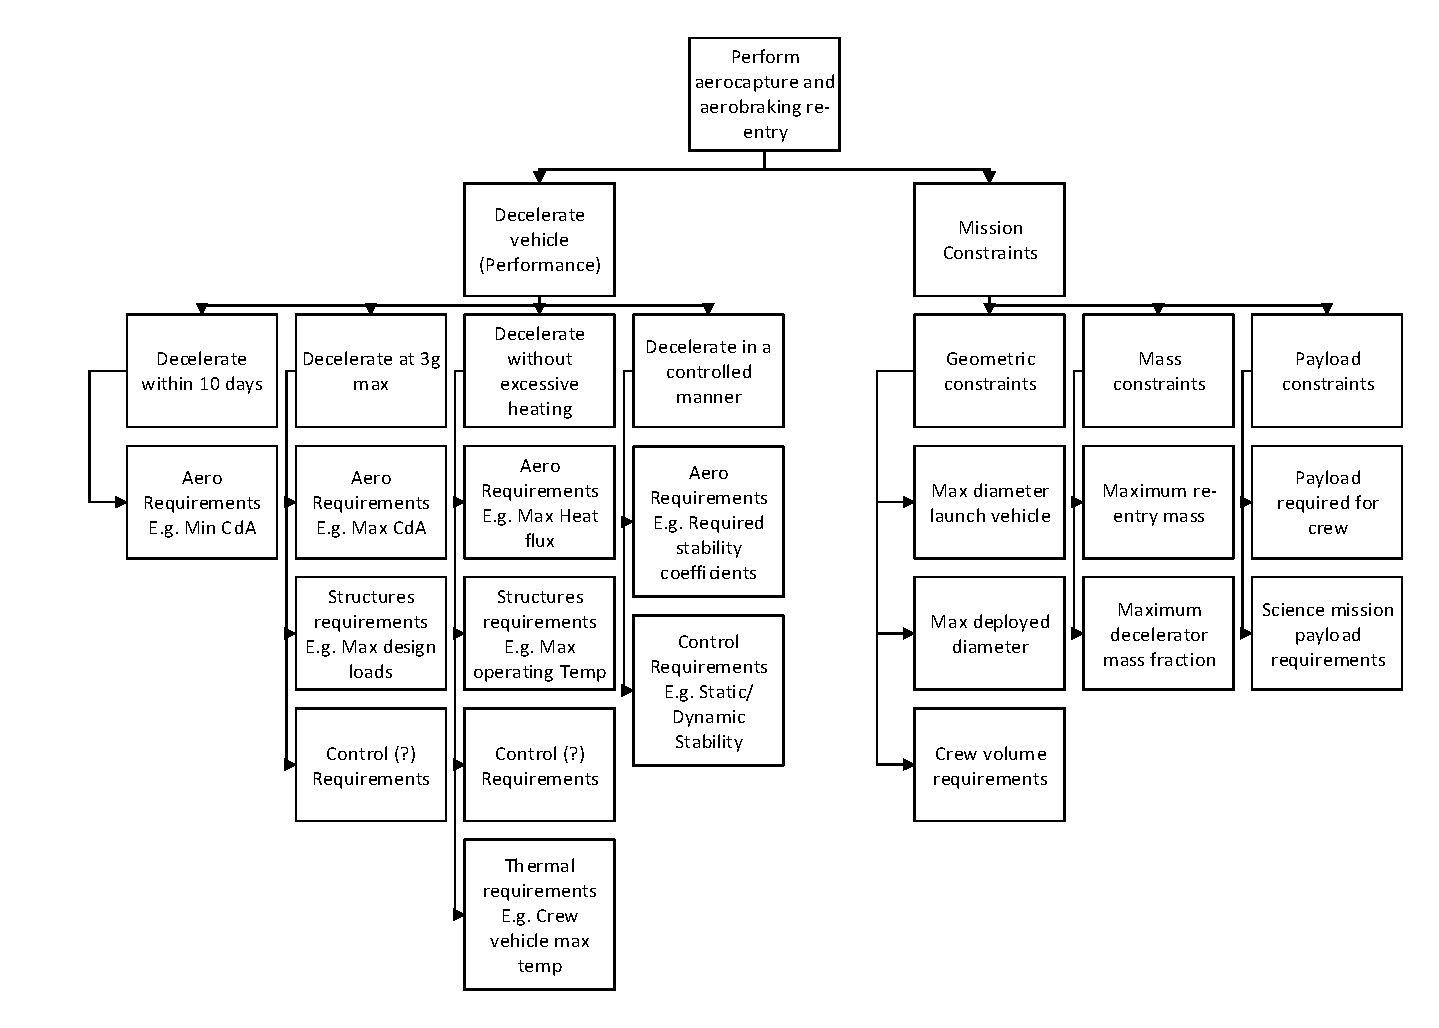
\includegraphics[width=0.95\textwidth]{./Figure/RBS.pdf}
\caption{Requirements Breakdown Structure} \label{fig:RBS}
\end{figure}

\subsection{Aerodynamic Requirements Discovery}

\subsection{Structural Requirements Discovery}

\subsection{Thermal Protection Requirements Discovery}

\subsection{Control & Orbital Requirements Discovery}

